%!TEX root = ../Thesis.tex


\section{GUI-Konzept}\label{GUI-Konzept}

Dieses GUI-Konzept entspricht dem Stand vor dem Beginn der Entwicklung unseres Prototypen.
Hilfreich war hierbei, dass zu diesem Zeitpunkt bereits die zu nutzenden Technologien festgelegt waren.
Für das Konzept, abgebildet in \cref{fig:gui-konzept}, wurde \enquote{Bootstrap 4}\footnote{\cite{bootstrap}} genutzt.
Hierdurch sind alle Buttons sowie UI-Elemente grundlegend einheitlich.
Dies findet sich insbesondere in der Navigationsleiste sowie den Buttons und Input-Feldern wieder.
Die Sprache ist auf Englisch gehalten, da Dies für uns am meisten gewohnt war.
Innerhalb der Navigationsleiste findet sich zur linken der Name unserer Anwendung sowie unser Logo.
Letzteres stellt stilisiert einen Regenschirm mit Funkverbindung da.
Eine humoristische Anspielung auf den Einsatzzweck unserer Anwendung.

\begin{figure}[h!!]
    \centering
    \begin{minipage}[t]{1\textwidth}
        \caption{GUI-Konzept}
        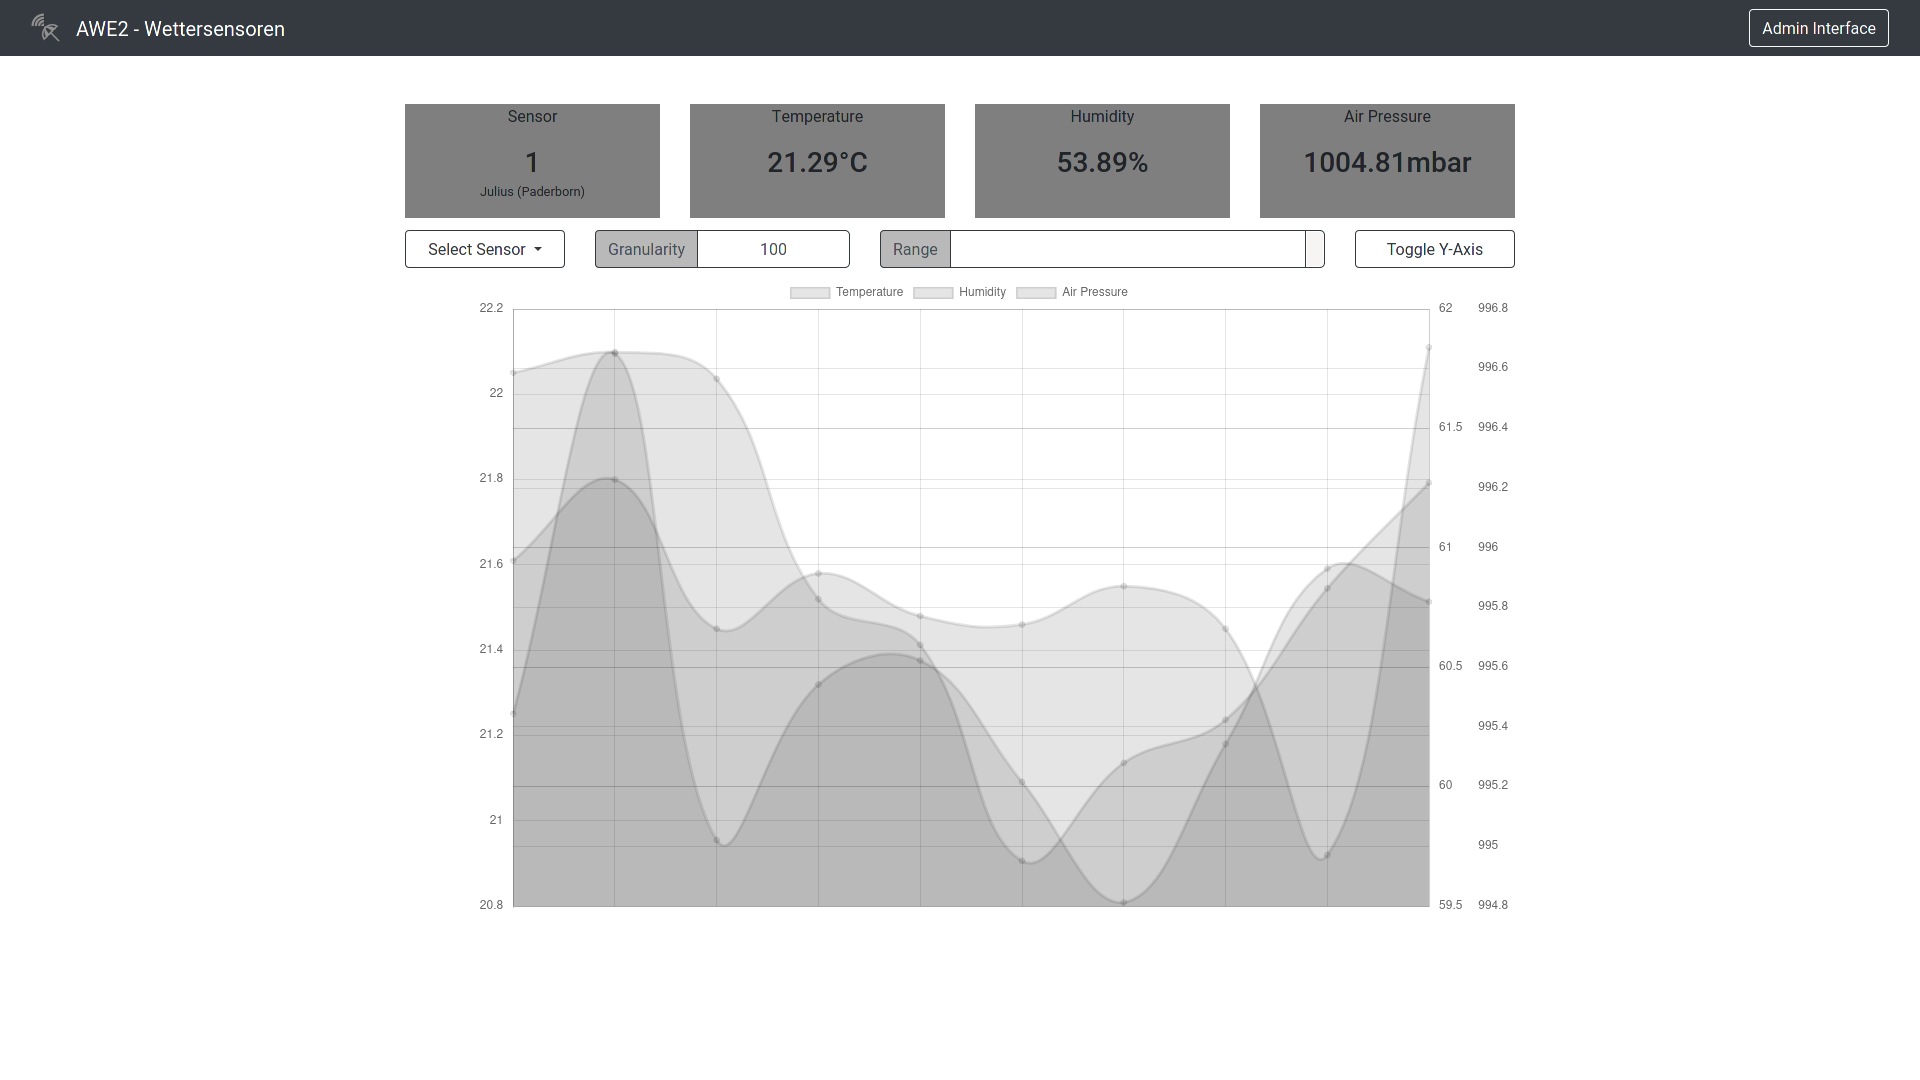
\includegraphics[width=1\textwidth]{img/gui-konzept.png}\\
        \source{Eigene Darstellung}
        \label{fig:gui-konzept}
    \end{minipage}
\end{figure}

Ziel unseres Konzeptes war es eine konsistente, einheitliche und leicht verständliche Benutzeroberfläche zu generieren.
Der Fokus unserer Anwendung ist die Darstellung und Auswertung von Wettersensoren. Unter diesen Aspekten wurde die Oberfläche entwickelt.
Informationen sind zentral gehalten, direkt ersichtlich sind vier Blöcke mittig auf dem Bildschirm platziert.
Durch diese ist einerseits der zurzeit ausgewählte Sensor andererseits alle drei aktuellen Sensorwerte im direkten Fokus des Anwenders.
Alle Einstellungsmöglichkeiten sind innerhalb einer darunterliegenden Reihe platziert.
Die Auswahl des darzustellenden Sensors erfolgt direkt unter der Ansicht des Aktuellen, auch hierdurch wird die Bedienung klar und für den Anwender einfach gehalten.
Daneben finden sich alle weiteren Eingabemöglichkeiten für Parameter der Graphen.
Das Hauptelement in Form der Graphen wird durch \enquote{chart.js}\footnote{\cite{chartjs.2020}} bereitgestellt.
Hier haben wir uns entschieden alle Sensorverläufe innerhalb eines Graphen zu plotten um Diese zentral und sichtbar zu halten.
Hier ist insbesondere anzumerken, dass Achsenbeschriftungen sowie Einfärbungen noch nicht vorhanden sind, da diese innerhalb des Codes durch Konfigurationen angepasst werden.

Durch die frühe Festlegung der Positionierung sowie der gesamten Oberfläche konnte sich während der Entwicklung auf die technische Implementierung konzentriert werden, da das fertige Design nur umgesetzt werden musste.
So war es im folgenden nur noch notwendig geringfügige Anpassungen vorzunehmen um der Anwendung den letzten Schliff zu geben.
Nach der Entwicklung des ersten Prototypen haben wir Dies einerseits in der Entwicklung eines einheitlichen Farbenkonzeptes umgesetzt.
Die in \cref{fig:farbmuster} abgebildeten Farben basieren in den hellen sowie dunklen Tönen auf Bootstrap Standart-Farben.
Für die weiteren Farbtöne haben wir uns eine Pastell-Farb-Palette ausgesucht. Diese wurden im folgenden einheitlich genutzt.
Der Gelbton wurde ausschließlich für Informationen benutzt, die restlichen Farben wurden jeweils für Temperatur, Luftfeuchte und Luftdruck genutzt.
Dies findet sich innerhalb der Blockelemente in der oberen Reihe aber auch insbesondere im Chart innerhalb der Graphen wieder, wo die Farben hervorhebend eingesetzt wurden.
Anderseits wurden die Informationen um passende \enquote{Font Awesome}-Icons\footnote{\cite{fontawesome}} ergänzt.
Hierdurch wird eine Orientierung auf der Oberfläche nochmals erleichtert und verbessert.
Darüber hinaus wurden die Block Elemente innerhalb der GUI um runde Kanten ergänzt, hierdurch bekam die Anwendung eine modernere zeitgemäßere Oberfläche. Die insbesondere konsistenter und passender zu den in Bootstrap vorhandenen Buttons ist.
\begin{figure}[h!!]
    \centering
    \begin{minipage}[t]{1\textwidth}
        \caption{Farben-Konzept}
        \includegraphics[width=0.5\textwidth]{img/Farbmuster.png}\\
        \source{Eigene Darstellung}
        \label{fig:farbmuster}
    \end{minipage}
\end{figure}

Die fertige GUI findet sich im Anhang \ref{gui-fertig}.
Weitere GUI-Elemente werden hier ebenfalls beschrieben.
Dazu gehören die Datumsauswahl in Anhang \ref{datumsauswahl}, das Admininterface im Anhang \ref{admininterface}, sowie die Informationsmeldungen im Anhang \ref{popup}.
Als netter Nebeneffekt ergab sich durch die Nutzung von Bootstrap, mit Hilfe geringer Anpassungen, eine nahezu vollständige Kompatibilität zu Mobilgeräten, auch wenn Diese nicht gefordert war.




